\documentclass[10pt,a4paper]{article}
\usepackage[utf8]{inputenc}
\usepackage[spanish]{babel}
\usepackage{amsmath}
\usepackage{amsfonts}
\usepackage{amssymb}
\usepackage{graphicx}
\usepackage[hidelinks]{hyperref}
\usepackage{listings}
\usepackage[left=2cm,right=2cm,top=2cm,bottom=2cm]{geometry}

\lstset { frame = single, breaklines = true }

\begin{document}

\begin{titlepage}
\title{\textbf{
	{\Huge Encapsular el acceso a una aplicación BASIC/MS-DOS}\\
	{\Large Sistemas Legados}
}}
\author{
	Pedro Allué Tamargo (758267)
	\and
	Juan José Tambo Tambo (755742)
	\and
	Jesús Villacampa Sagaste (755739)
}
\date{\today}
\clearpage\maketitle
\thispagestyle{empty}
\tableofcontents
\end{titlepage}


\section{Introducción}

En esta práctica se pide la realización de un \emph{wrapper} sobre una aplicación legada de un sistema \emph{MS-DOS}. Para ello se va a utilizar un emulador y mediante capturas de pantallas de la interacción con la misma y un software de reconocimiento de caracteres (\emph{OCR}) se van a extraer los datos.


\section{Esfuerzos invertidos}

\begin{itemize}
\item Pedro Allué Tamargo:
\item Juan José Tambo Tambo:
\item Jesús Villacampa Sagaste:
\end{itemize}

\section{Descripción de la aplicación legada}

Para interaccionar con la aplicación legada se va a utilizar el emulador \emph{DosBox} (el incluido junto al enunciado de la práctica). Para ejecutar la aplicación se va a ejecutar el \emph{script} \texttt{database.bat} que ejecuta el emulador y la aplicación legada.\\
La aplicación legada consiste en un programa de \emph{MS-DOS} que gestiona una biblioteca de cintas con distintos programas y/o juegos (Figura \ref{fig:aplicacion_legada}).

\begin{figure}[h!]
\centering
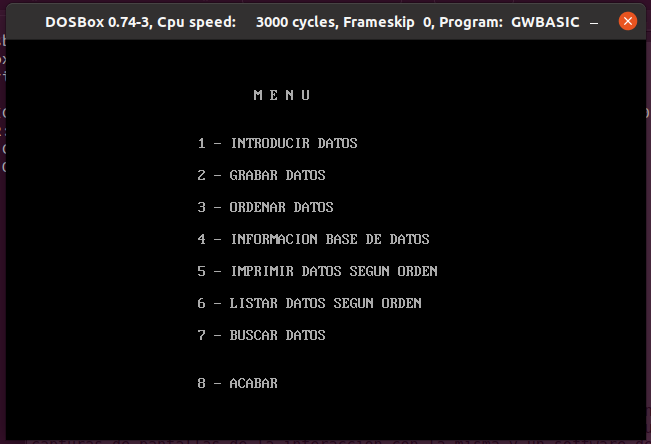
\includegraphics[scale=0.5]{images/aplicacion_legada.png}
\caption{Captura de pantalla del menú principal de la aplicación legada}
\label{fig:aplicacion_legada}
\end{figure}

Con esta aplicación el usuario podía introducir nuevos registros que hacían alusión a cintas con los campos: \emph{Nombre}, \emph{Tipo}, \emph{Cinta}. También se añade un campo que gestiona la propia aplicación correspondiente al número de registro que le corresponde en la base de datos.


\section{Tecnología elegida}

Se ha elegido \emph{Java} como lenguaje de programación para esta tarea. Para implementar el servidor web se ha utilizado el \emph{framework SpringBoot} por su facilidad de uso. Se va a utilizar un servidor de aplicaciones \emph{Apache Tomcat} incluido en el \emph{framework} de \emph{Spring}. Se va a exponer una API REST para obtener los datos del servidor.\\
Para la creación de la página web y la interacción con la \emph{API REST} del servidor se va a utilizar \emph{Vue.js}, un \emph{framework} de \emph{JavaScript}.\\

\section{Implementación del Wrapper}
\subsection{Preparación del entorno}

Para la realización de esta práctica se va a utilizar el sistema operativo \emph{Ubuntu}, se debe instalar el emulador \emph{DosBox}. Para ello se ejecutarán las siguientes órdenes:

\begin{lstlisting}
sudo apt update
sudo apt -y install dosbox
\end{lstlisting}


En primer lugar se deberá configurar el emulador \emph{DosBox} para que monte el directorio de la aplicación legada en un disco virtual (\emph{C}) y para que ejecute el programa. Para ello se añadirán las siguientes líneas al fichero de configuración ubicado en el directorio \texttt{\$HOME/.dosbox}. Se añadirán las siguiente líneas al fichero de configuración (\texttt{dosbox-0.74-3.conf}) en la sección \texttt{[autoexec]}:

\begin{lstlisting}
[autoexec]
# Lines in this section will be run at startup.
# You can put your MOUNT lines here.

MOUNT C $HOME/.dosbox/c/
C:
cd Database
GWBASIC.BAT
\end{lstlisting}

Tras eso se va a proceder a crear el directorio \texttt{\$HOME/.dosbox/c} con el contenido de la aplicación legada.\\

Para poder utilizar el reconocimiento de caracteres (\emph{OCR}) se debe instalar la librería \emph{Tesseract} para el Sistema Operativo. Para instalarla se ejecutarán los siguientes comandos:

\begin{lstlisting}
sudo apt update
sudo apt -y install tesseract-ocr
\end{lstlisting}

De cara al reconocimiento de caracteres en las capturas de pantallas se va a utilizar otro binario para conseguir la posición de la ventana del emulador. Se va a proceder a instalar el binario \emph{wmctrl}. Para ello se ejecutarán las siguientes órdenes:

\begin{lstlisting}
sudo apt update
sudo apt -y install wmctrl
\end{lstlisting}


\subsection{Frontend del Wrapper}

Para la realización de la parte del \emph{frontend} se ha utilizado \emph{Vue.js}, un \emph{framework} de \emph{JavaScript} de código abierto que permite la construcción de interfaces de usuario de una manera sencilla y agradable. \\ 
Este \emph{framework} nos permite mostrar el contenido de manera dinámica en la página web a través de llamadas a la \emph{API REST} del servidor.\\
Para la elaboración del código en \emph{HTML}, se ha utilizado la herramienta \emph{Bootstrap}, de código abierto y de uso gratuito que dispone de plantillas \emph{HTML} y \emph{CSS} para interfaces de usuario que permite que éstas sean usables y accesibles. Esta herramienta cuenta con plantillas de todo tipo desde distintas estructuras como pueden ser listas, tablas, filas o columnas hasta botones ya diseñados, lo que ha permitido que la implementación haya sido tanto poco costosa como intuitiva para el usuario.\\
Para el proceso de desarrollo se ha utilizado la herramienta \texttt{npm}, que es un gestor de dependencias de \emph{JavaScript}. Sirve para instalar y gestionar versiones de paquetes y librerías, y permite ver en tiempo real el resultado de la página web en un navegador web tan solo guardando los cambios efectuados en el código.\\

\textbf{Metemos captura de como queda la página??? SI}\\

Para integrar este \emph{frontend} con el código del servidor de \emph{backend} se ha creado un \emph{script BASH} para compilar y copiar el resultado de este proyecto al servidor \emph{backend}. El código del \emph{script} es el mostrado en el código \ref{list:copyToTomcat}.

\lstinputlisting[language=sh, label=list:copyToTomcat]{listings/copyToTomcat.sh}

\subsection{Backend del Wrapper}

\textbf{Rellenar con el desarrollo del backend}


\end{document}